\section{The dataset features}

\subsection*{The Rapidity-Mass matrix (RMM) }\label{sec:rmm}
Most of the features in the analysis are elements in the so called Rapidity-Mass matrix (RMM)  inspired by the work of Chekanov \cite{Chekanov_2019}.
\par
The RMM is a convenient structure to create a feature space for the dataset. It contains information of various reconstructed objects and their combinations 
about mass, rapidity, momenta and missing transverse energy, all of which are useful in searches for new physics\cite{Chekanov_2021} in HEP. 
One example of an analysis that have used some of the features from the RMM is demontrated in \cite{Santos_2017}. The main reason however 
for using this structure is the systematic layout and automated featurespace, that maintains low to no corrolation between the cells in the 
matrix, as this is ideal when using neural networks.
\par
Its composition is determined as a square matrix of $1 + \sum_{i=1}^{T}N_i$ columns and rows, where T is the total number of objects (i.e jets, 
electrons etc.), and $N_i$ is the multiplicity of a given object. In the case of the same number of a given object for all objects, we can 
denote the RMM matrix as a TmNn matrix, where m is the multiplicity of T, and n is the number of particle per type. Thus there is already 
room for evaluation, as the combination of number of objects and the number of each object type highly affects the analysis as well as 
computational resources. Each cell in the matrix contains information about either single og two particle properties. This could in principle be
generalized to three particle properties, which would make a three dimensional RMM. The scope of thesis will for simplicity only cover the 
two dimensional case. An example is 
shown in matrix \ref{eq:rmmmatrix}.

\begin{equation}\label{eq:rmmmatrix}
\begin{pmatrix}
    \boldsymbol{e}_{T}^{miss} & m_T(j_1) & m_T(j_2) &  m_T(e_1) &  m_T(e_2)\\
    h_L(j_1) & \boldsymbol{e_T}(j_1) & m(j_1, j_2) & m(j_1, e_1) & m(j_1, e_2)\\
    h_L(j_2) & h(j_2, j_1) & \delta \boldsymbol{e_T}(j_2)& m(j_2, e_1) & m(j_2, e_2)\\
    h_L(e_1) & h(e_1, j_1) & h(e_1, j_2) & \boldsymbol{e_T}(e_1) & m(e_1, e_2)\\
    h_L(e_2) & h(e_2, j_1) & h(e_2, j_2) & h(e_2, e_1) & \delta \boldsymbol{e_T}(e_2)\\
\end{pmatrix}
\end{equation}

In matrix \ref{eq:rmmmatrix} we have the RMM matrix for a T2N2 system, in other words we have two types of particles, jets
\footnote{Jets here can both be b- or ljets. Ljet is defined as jets with jetdl1r < 0.665, where as bjet77 is defined as jets with jetdl1r>=2.195, 
where jetdl1r is a machine learning output from a network trained to destinguish b- and ljets.} and electrons, where each type has two particles. 
The matrix itself is partitioned into three parts. 
The diagonal represents energy properties, the upper triangular represents mass properties, and the lower triangular represents longitudal 
properties related to rapidity. The diagonal has three different properties, $\boldsymbol{e_T^{miss}}$, $\boldsymbol{e_T}$ and $\delta\boldsymbol{e_T}$. 
$\boldsymbol{e_T^{miss}}$ is placed in the $(0,0)$ position in the matrix. It accounts for the missing transverse energy for the system, which is of 
high interest for this analysis due to the search for heavy neutrinos. $\boldsymbol{e_T}$ is the transverse energy defined as 

\begin{equation}\label{eq:et}
    \boldsymbol{e_T} = \sqrt{m^2 + p_T^2}
\end{equation}
but for light particles such as electrons, this can be approximated to $\boldsymbol{e_T} \approx p_T$. $\delta\boldsymbol{e_T}$ 
is the transverse energy imbalance. It is defined as 
\begin{equation}\label{eq:deltaet}
    \delta\boldsymbol{e_T} = \frac{E_T(i_n-1) - E_T(i_n)}{E_T(i_n-1) + E_T(i_n)}, \, n = 2, ..., N.
\end{equation}
The first columm in the RMM matrix, with the exeption of the first element, is related to the longitudal property of the given particle. 
It is defined as
\begin{equation*}
    h_L(i_n) = C(\cosh{(y)} - 1),
\end{equation*}
where C is a constant to ensure that the average $h_L(i_n)$ values do not deviate too much from the ranges of the invariant masses 
of the transverse masses, found to be $0.15$, as it ensures that rapidity ranges in the range $[-2.5, 2.5]$ produces $h_L(i_n)$ values in the 
$[0,1]$ interval\cite{Chekanov_2019}. y is the rapidity of the particle, and $i_n$ is the particle number. 
On the lower triangle we have the longitudal properties of the combinations of particles. Similar to $h_L(i_n)$, this property is defined as 
\begin{equation*}
    h(i_n, j_k) = C(\cosh{(\Delta y)} - 1),
\end{equation*}
where $\Delta y = y_{i_n} - y_{j_k}$ is the rapidity difference for particle $i_n$ and $j_k$. 


\subsection*{Tabular and sparce data}
A concequence of using the RMM structure is that the data and Monte Carlo are sparce. This is due to the fact that the RMM allows for 
the variaty of final states of the reconstructed events, i.e that one event has two ljets, zero bjets, one electron and two muons, where as another 
event can have 4 ljet, 3 bjets and three electrons. This means that the RMM matrix for each event will have a different size, 
and for neural networks this is a problem. To solve this problem, Chekanov simply pads the missing values with 0s\cite{Chekanov_2019}. 

\subsection*{MonteCarlo and data comparison}\label{sec:mcdatacomp}

Before we can start the analysis, we need to compare the MonteCarlo and data. This is done to ensure that the measured features used 
are reconstructed well by the MonteCarlo training samples we use. As described by R. Stuart Geiger et al. \cite{DBLP:journals/corr/abs-2107-02278}, the concept of "Garbage 
in, garbage out" is of key importance in computer science, and indeed important in high energy physics. To ensure that the models 
we train actually learn physical processes, the training set must represent the physics "status quo". If the training samples do 
not match the physical reality, we regard it, in the context of high energy physics, as garbage in, which will in turn give 
garbage out. The Monte Carlo standard model simulations are indeed very good, but they are numerical approximations, and can 
sometimes be off. Thus, every feature that will be used for training have to be checked before being used. This is done by 
comparing the distributions of the features in the MonteCarlo and ATLAS data. MonteCarlo simulations are based on the actual theory 
itself, and comparisons with data taken from ATLAS and other detectors alike are neccesary to prove that the standard model is a good model.

Now, if we compare all SM MonteCarlo and ATLAS data, we would usually expect there to be a good overlap. To ensure that the standard model 
MonteCarlo actualy represents the physics, we create signal and background regions to optimize for a signal and or background. If we can 
create a background region where we believe with very high certainty that only standard model processes can occur, and we get a good match, 
we usually conclude that the MonteCarlo is good enough. Now, for this thesis, simply comparing all ATLAS data to all standard model MonteCarlo
is enough, as this data batch has been analysed by the ATLAS collaboration for multiple years without finding any new physics, concluding 
that if the signals are there, they are too small for so called visual cuts. Traditional searches have only exluded some models, which is why 
machine learning is getting more popular. The hope is that the signal, whatever it might be, can be revealed with clever feature 
engineering and smart machine learning algorithms. Particle physics differs here from more day to day machine learning as the target data is 
unlabeled. 


\begin{figure}[h!]
    \centering
    \begin{subfigure}{.6\textwidth}
        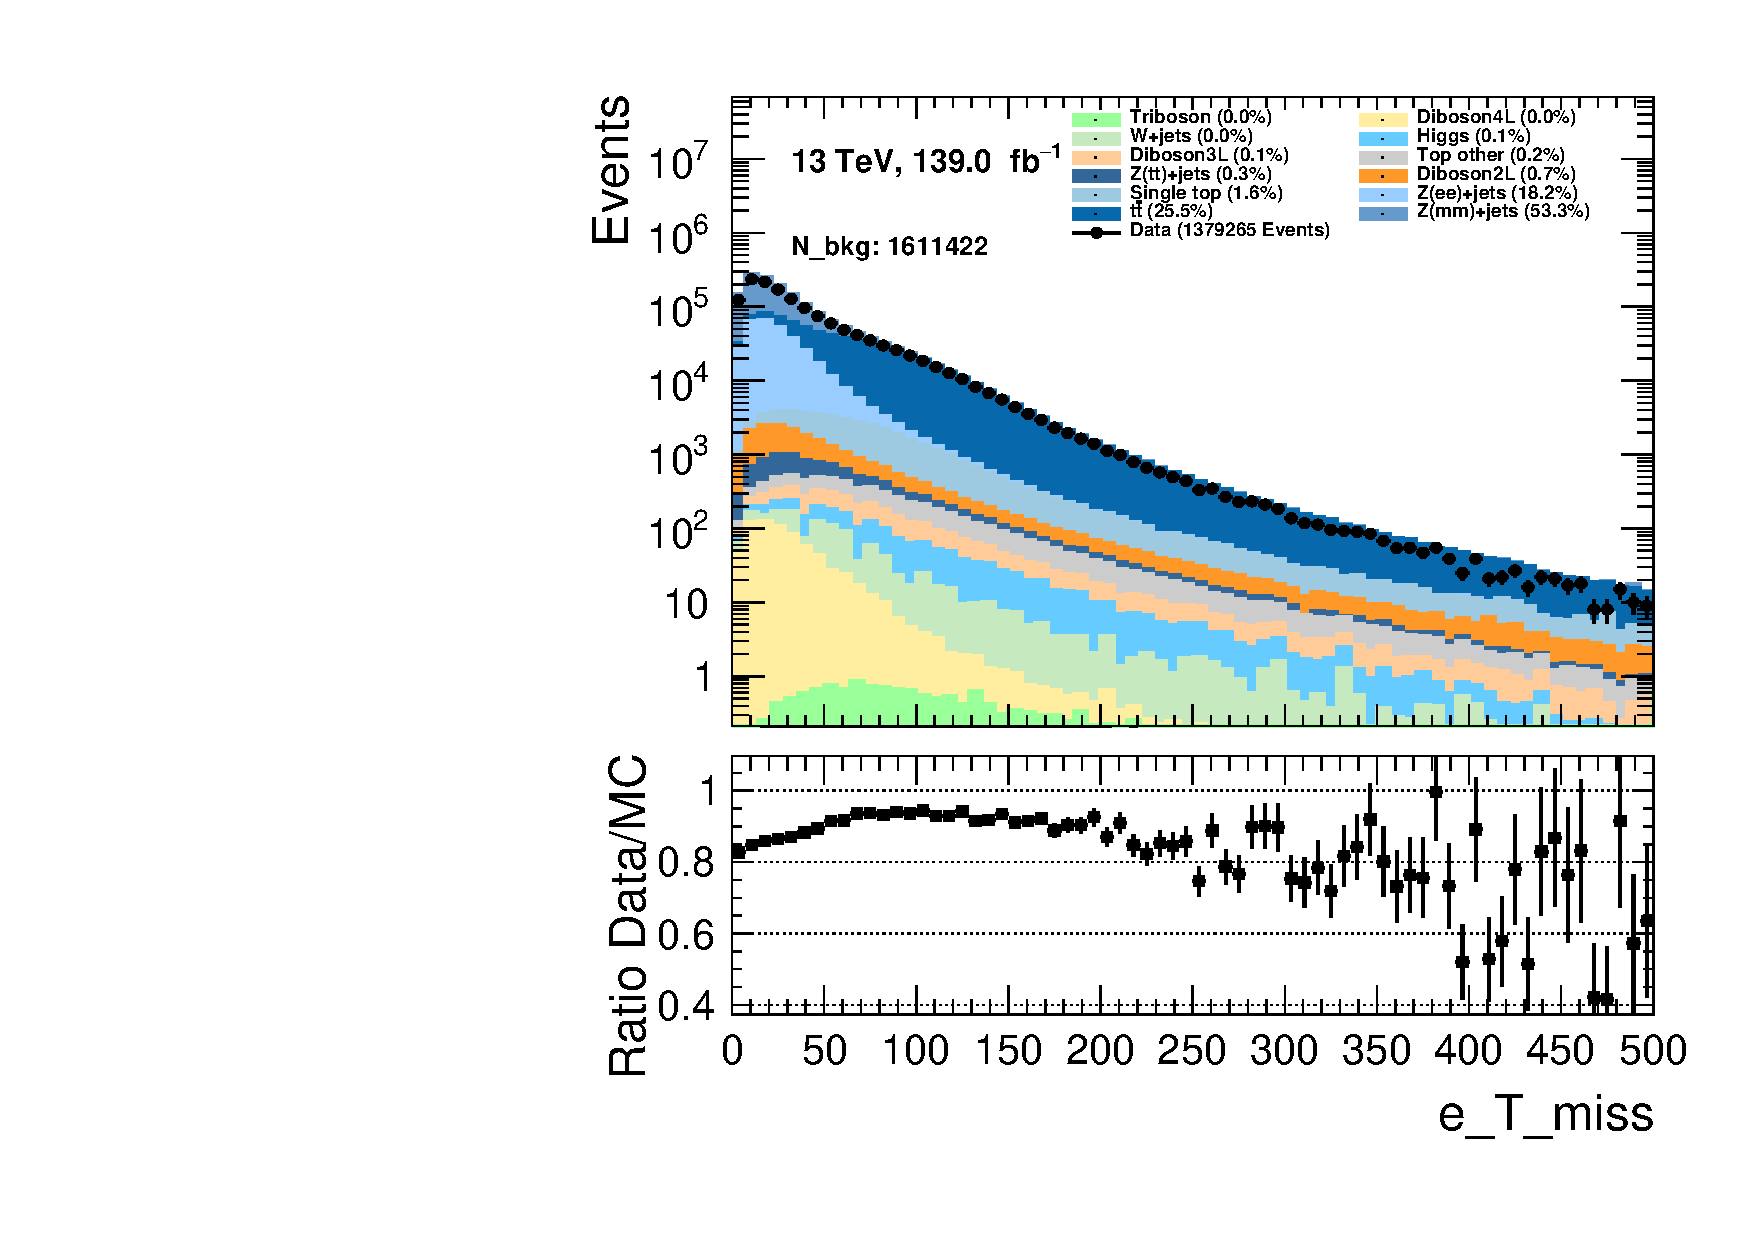
\includegraphics[width=\textwidth]{Figures/MC_Data_comp/lep3/e_T_miss_3lep.pdf}
        \caption{Missing transverse energy for the three lepton final state in GeV. The histogram contains the entire Run 2 dataset.}
        \label{fig:etmiss}
    \end{subfigure}
    \hfill
    \begin{subfigure}{.6\textwidth}
        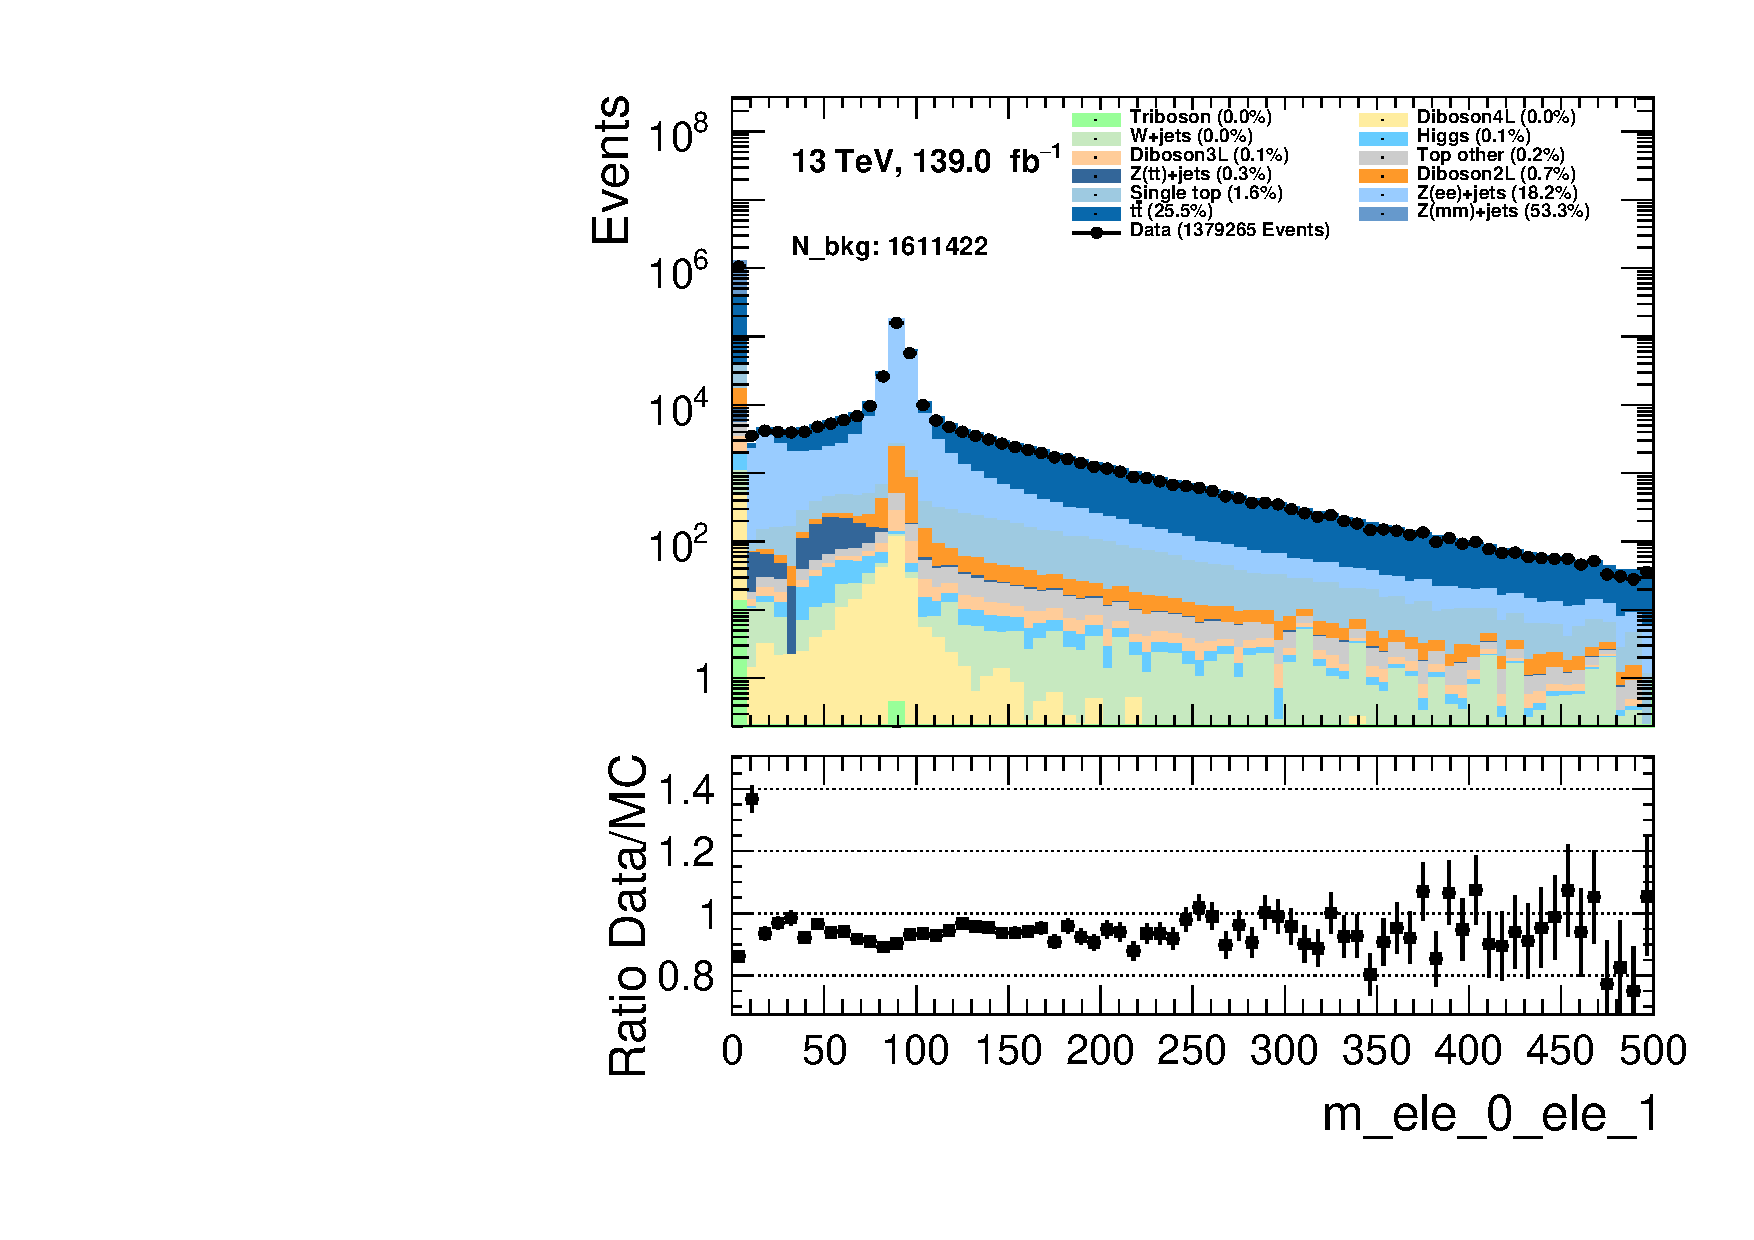
\includegraphics[width=\textwidth]{Figures/MC_Data_comp/lep3/m_ele_0_ele_1_3lep.pdf}
        \caption{Invariant mass for the first and second electron in GeV. The histogram contains the entire Run 2 dataset. }
        \label{fig:mll_3lep}
    \end{subfigure}
    \hfill        
    \caption[3 lepton + $e_T^{miss}$ MonteCarlo and ATLAS data comparison]{Comparison of the MonteCarlo and data for the three lepton + $e_T^{miss}$ final state with the features $e_{T}^{miss}$ and flavor composition.
    }
    \label{fig:MC_Data_comp}
\end{figure}

In figure \ref{fig:MC_Data_comp} two features have been selected to vizualize the comparison between Monte Carlo and ATLAS data, $e_T^{miss}$ 
and $m(ele_0, ele_1)$ in the 3 lepton + $e_T^{miss}$ dataset. We see that both $e_T^{miss}$ and $m(ele_0, ele_1)$ satisfy a good ratio between Monte Carlo and ATLAS data, thus we can safely 
move forward with the analysis. All features were checked, and can be found in the Github repository for this thesis at 
\href{https://github.com/Gadangadang/MasterThesis/tree/main}{Figures/Histo\_var\_check}\footnote{Full link: \href{https://github.com/Gadangadang/MasterThesis/tree/main/Figures/histo_var_check/LEP3}{$https://github.com/Gadangadang/MasterThesis/tree/main/Figures/histo\_var\_check/LEP3$}} under the 3lep folder. \par 

\begin{figure}[h!]
    \centering
    \begin{subfigure}{.6\textwidth}
        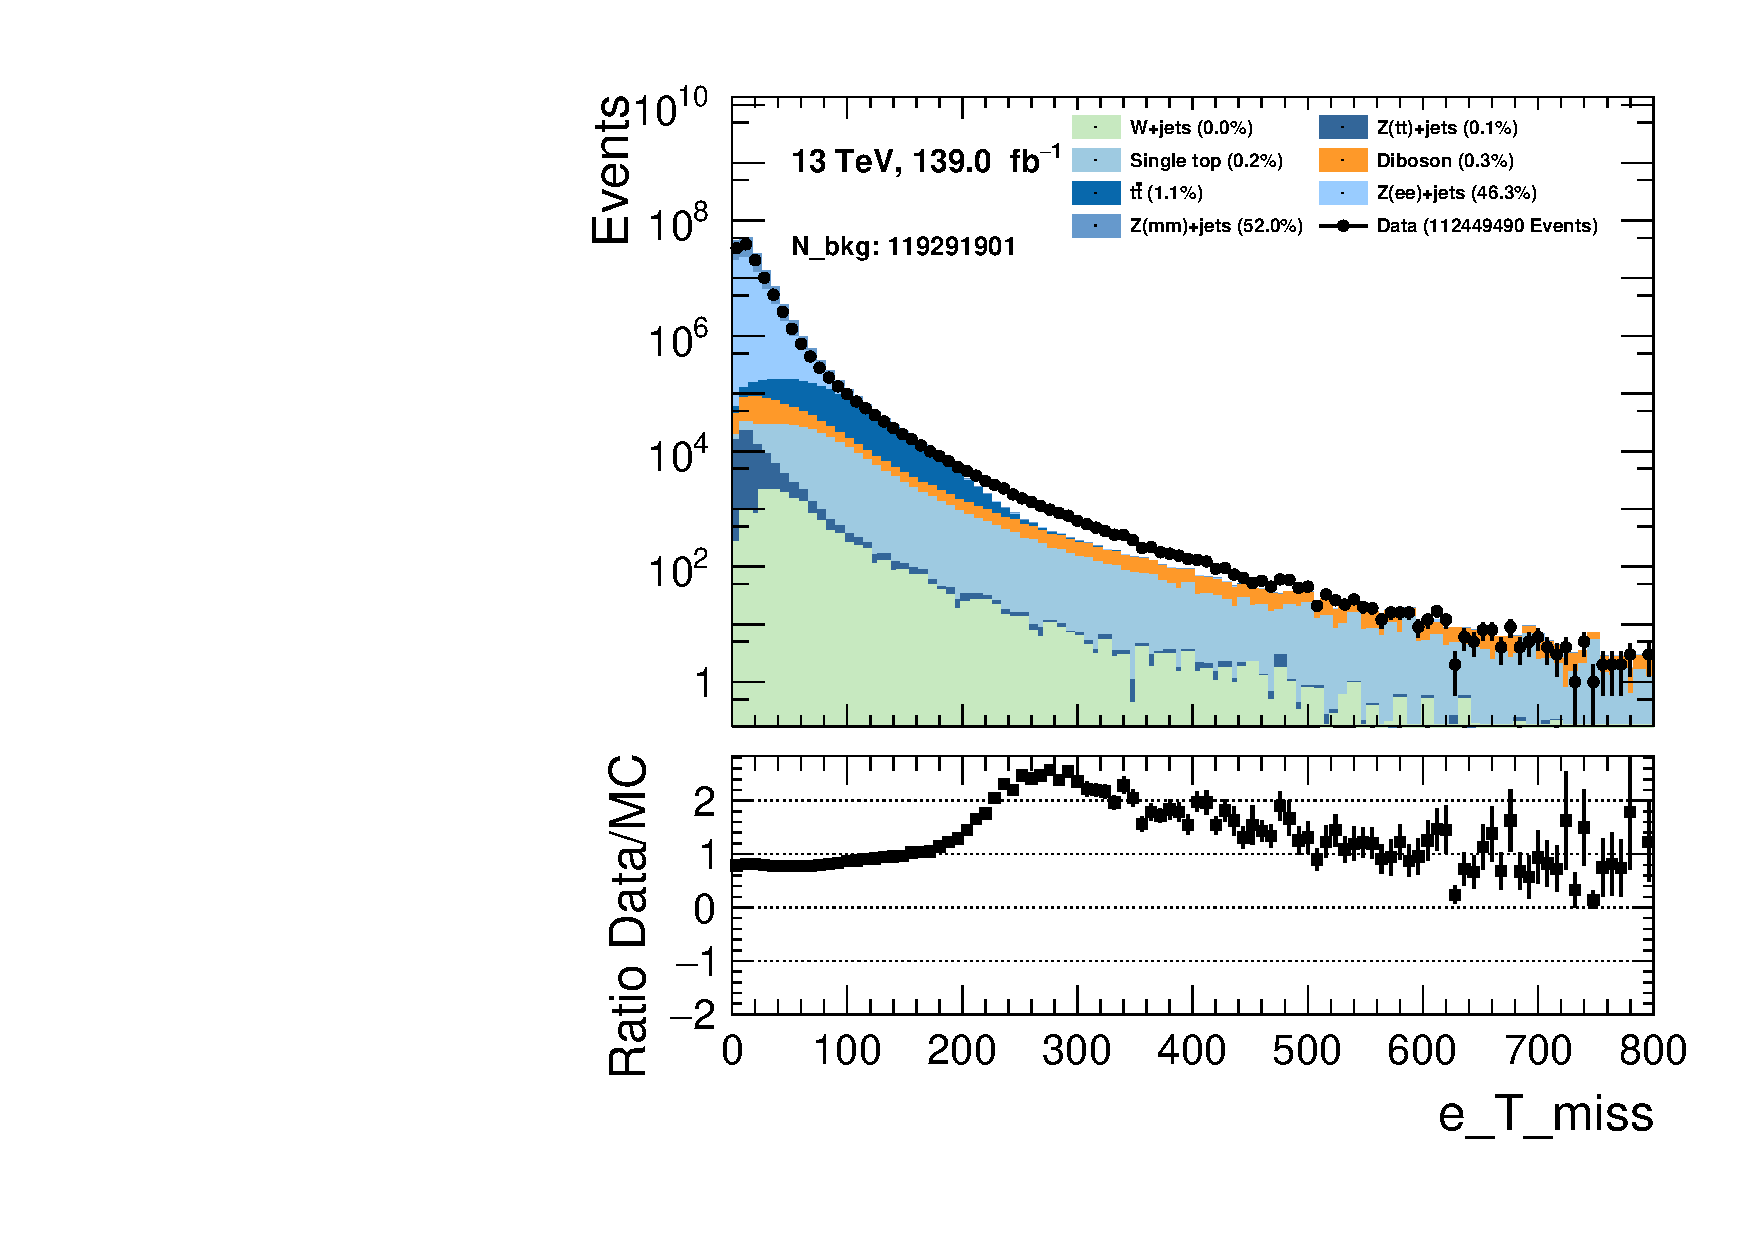
\includegraphics[width=\textwidth]{Figures/MC_Data_comp/lep2/e_T_miss_2lep.pdf}
        \caption{Missing transverse energy for the three lepton final state in GeV. The histogram contains the entire Run 2 dataset. Note here the lack of good overlap from about
        200-500 GeV.}
        \label{fig:etmiss_2lep}
    \end{subfigure}
    \hfill
    \begin{subfigure}{.6\textwidth}
        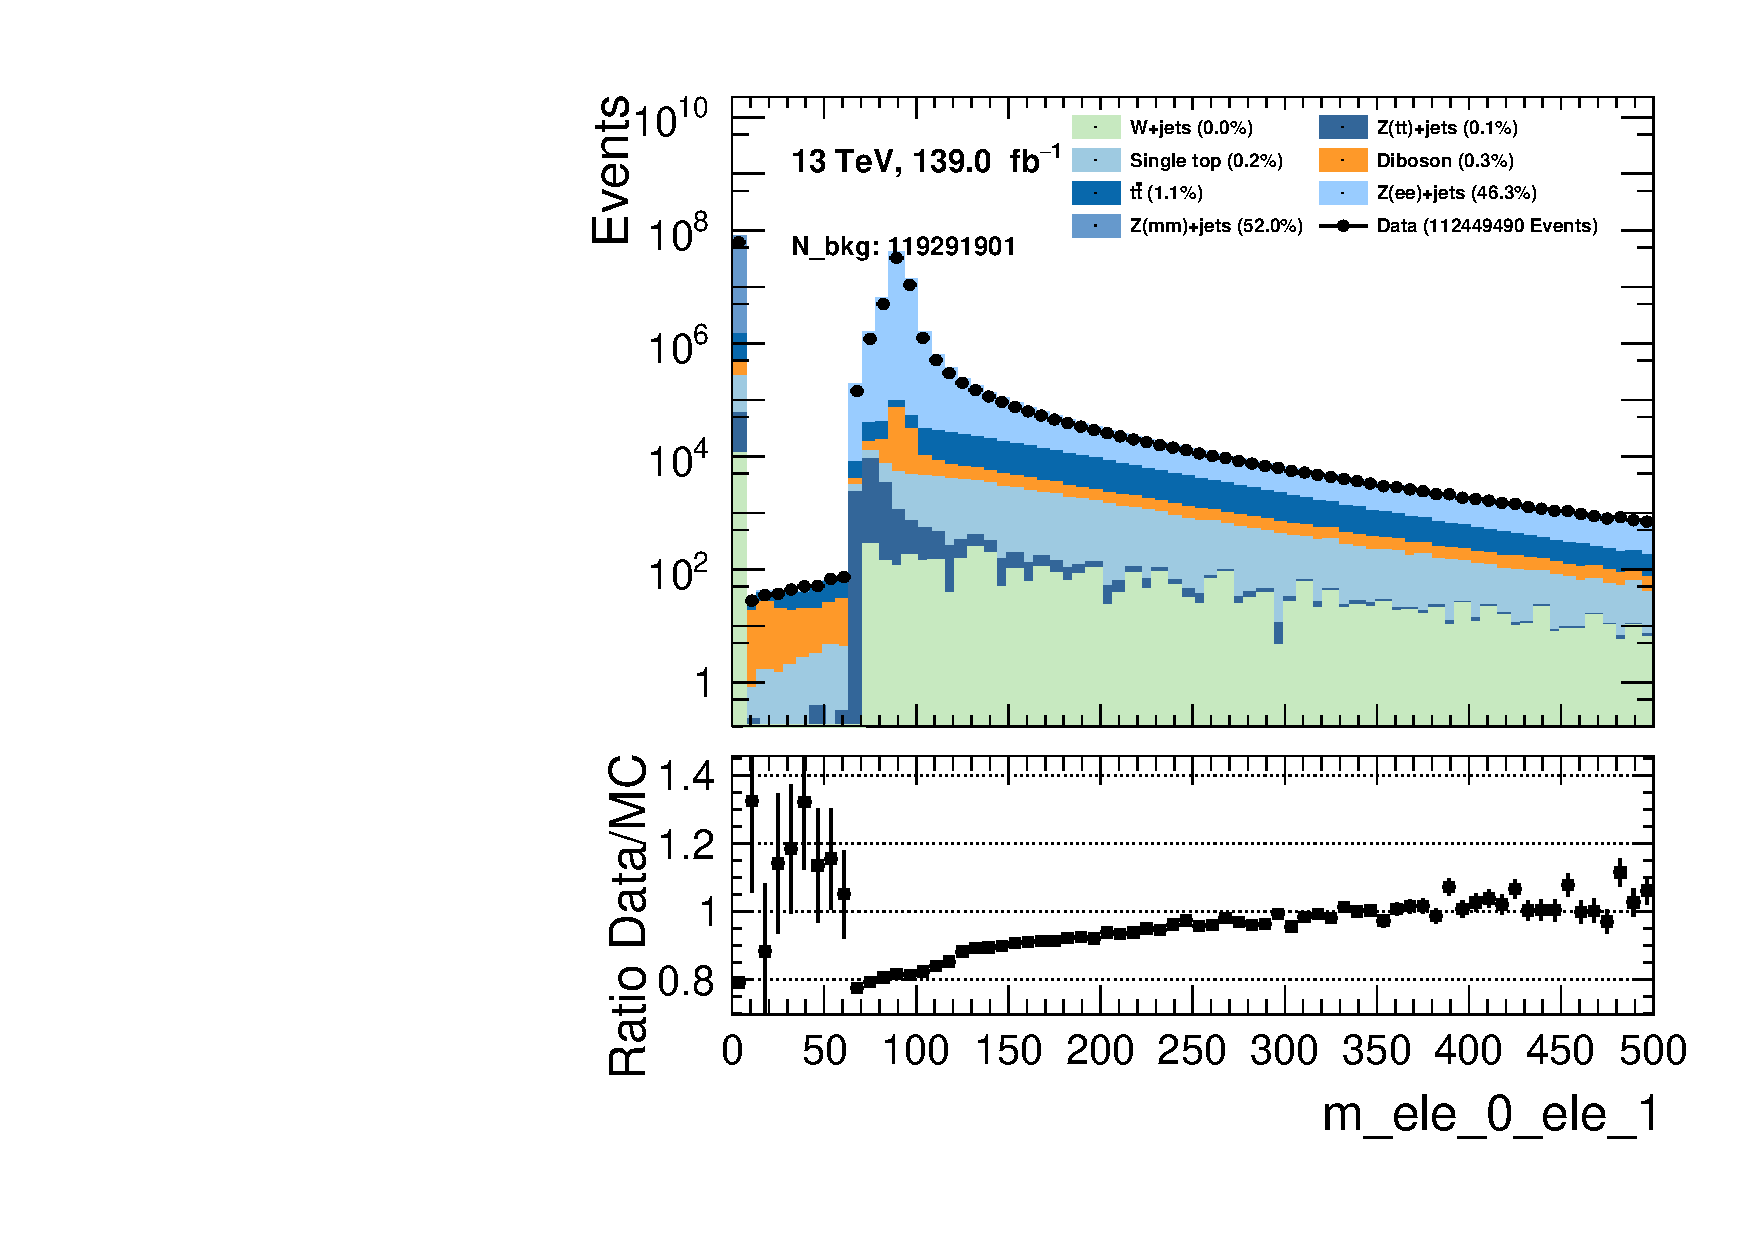
\includegraphics[width=\textwidth]{Figures/MC_Data_comp/lep2/m_ele_0_ele_1_2lep.pdf}
        \caption{Invariant mass for the first and second electron in GeV. The histogram contains the entire Run 2 dataset. Note the sharp reduction of events from 10-70 GeV.}
        \label{fig:mll_2lep}
    \end{subfigure}
    \hfill        
    \caption[2 lepton + $e_T^{miss}$ MonteCarlo and ATLAS data comparison]{Comparison of the MonteCarlo and data for the 2 lepton + $e_T^{miss}$ final state with the features $e_{T}^{miss}$ and flavor composition.
    }
    \label{fig:MC_Data_comp_2lep}
\end{figure}
The same checks were done for the 2 lepton + $e_T^{miss}$ dataset. In figure \ref{fig:MC_Data_comp_2lep} we see that the features $e_T^{miss}$ and $m(ele_0, ele_1)$ 
do not satisfy the same ratio between SM MC and ATLAS data, as with the 3 lepton + $e_T^{miss}$ case. It is suspected that the trigger matching and 
triggers are not implemented properly, but neither the author or the supervisors have found a solution to the issue, and due to time constraints, chose to 
move forward with the analysis regardless. Thus, for all results regarding the 2 lepton + $e_T^{miss}$ dataset should be interpreted with this in mind. One attempt can be shown in 
figure \ref{fig:mll_2lep} where a cut on the invariant mass above 70 GeV of at least the two leptons with the highest energy, to try to acommodate the trigger issue. 
It did not seem to work. All features were checked, and can be found in the Github repository for this thesis at 
\href{https://github.com/Gadangadang/MasterThesis/tree/main}{Figures/Histo\_var\_check}\footnote{Full link: \href{https://github.com/Gadangadang/MasterThesis/tree/main/Figures/histo_var_check/LEP2}{$https://github.com/Gadangadang/MasterThesis/tree/main/Figures/histo\_var\_check/LEP2$}} under the 2lep folder.



\subsubsection*{Triggers }\label{sec:triggers}
The following triggers where implemented for the 2 lepton + $e_T^{miss}$  and 3 lepton + $e_T^{miss}$ dataset are written below:



   

\begin{table}[h!]
    \centering
    \caption[2015 triggers table]{Triggers used in the 2015 MonteCarlo and ATLAS data samples for the 2 lepton 0 $e_T^{miss}$ dataset.}
\begin{tabular}{|l|l|l|}
\hline
                      & Name & Description \\ \hline
\multirow{6}{*}{2015} & $HLT\_2e15\_lhvloose\_nod0\_L12EM13VH$      &             \\ \cline{2-3} 
                      & $HLT\_2e12_lhloose_L12EM10VH$      &             \\ \cline{2-3} 
                      & $HLT\_2mu10$     &             \\ \cline{2-3} 
                      & $HLT\_mu18\_mu8noL1$      &             \\ \cline{2-3} 
                      & $HLT\_e17\_lhloose\_mu14$    &             \\ \cline{2-3} 
                      & $HLT\_e7\_lhmedium\_mu24$      &             \\ \hline
\end{tabular}
\end{table}



\begin{table}[h!]
    \centering
    \caption[2016 triggers table]{Triggers used in the 2016 MonteCarlo and ATLAS data samples for the 2 lepton 0 $e_T^{miss}$ dataset.}
    \begin{tabular}{|l|l|l|}
    \hline
                          & Name & Description \\ \hline
    \multirow{9}{*}{2016} & $HLT\_2e15\_lhvloose\_nod0\_L12EM13VH$      &             \\ \cline{2-3} 
                          & $HLT\_2e17\_lhvloose\_nod0$      &             \\ \cline{2-3} 
                          & $HLT\_2mu10$     &             \\ \cline{2-3} 
                          & $HLT\_2mu14$     &             \\ \cline{2-3} 
                          & $HLT\_mu20\_mu8noL1$     &             \\ \cline{2-3} 
                          & $HLT\_mu22\_mu8noL1$      &             \\ \cline{2-3} 
                          & $HLT\_e17\_lhloose\_nod0\_mu14$      &             \\ \cline{2-3} 
                          & $HLT\_e24\_lhmedium\_nod0\_L1EM20VHI\_mu8noL1$     &             \\ \cline{2-3} 
                          & $HLT\_e7\_lhmedium\_nod0\_mu24$      &             \\ \hline
    \end{tabular}
    \end{table}




\begin{table}[h!]
    \centering
    \caption[2017 triggers table]{Triggers used in the 2017 MonteCarlo and ATLAS data samples for the 2 lepton 0 $e_T^{miss}$ dataset.}
    \begin{tabular}{|l|l|l|}
    \hline
                            & Name & Description \\ \hline
    \multirow{7}{*}{2017} & $HLT\_2e17\_lhvloose\_nod0\_L12EM15VHI$      &             \\ \cline{2-3} 
                            & $HLT\_2e24\_lhvloose\_nod0$        &             \\ \cline{2-3} 
                            & $HLT\_2mu14$     &             \\ \cline{2-3} 
                            &  $HLT\_mu22\_mu8noL1$     &             \\ \cline{2-3} 
                            &  $HLT\_e17\_lhloose\_nod0\_mu14$   &             \\ \cline{2-3} 
                            &   $HLT\_e26\_lhmedium\_nod0\_mu8noL1$    &             \\ \cline{2-3} 
                            
                            & $HLT\_e7\_lhmedium\_nod0\_mu24$    &  \\ \hline
    \end{tabular}
    \end{table}


    \begin{table}[h!]
        \centering
        \caption[2018 triggers table]{Triggers used in the 2018 MonteCarlo and ATLAS data samples for the 2 lepton 0 $e_T^{miss}$ dataset.}
        \begin{tabular}{|l|l|l|}
        \hline
                                & Name & Description \\ \hline
        \multirow{7}{*}{2018} & $HLT\_2e17\_lhvloose\_nod0\_L12EM15VHI$      &             \\ \cline{2-3} 
                                & $HLT\_2e24\_lhvloose\_nod0$        &             \\ \cline{2-3} 
                                & $HLT\_2mu14$     &             \\ \cline{2-3} 
                                &  $HLT\_mu22\_mu8noL1$     &             \\ \cline{2-3} 
                                &  $HLT\_e17\_lhloose\_nod0\_mu14$   &             \\ \cline{2-3} 
                                &   $HLT\_e26\_lhmedium\_nod0\_mu8noL1$    &             \\ \cline{2-3} 
                                
                                & $HLT\_e7\_lhmedium\_nod0\_mu24$    & \\ \hline
        \end{tabular}
        \end{table}












